\documentclass[conference]{IEEEtran}
\raggedbottom
\hbadness=4000

\usepackage[T1]{fontenc}
\usepackage[utf8]{inputenc}
\usepackage{amsmath,amssymb}
\usepackage{booktabs}
\usepackage{tabularx}
\usepackage{array}
\usepackage{graphicx}
\usepackage{xcolor}
\usepackage{hyperref}
\usepackage{microtype}

\hypersetup{
  colorlinks=true,
  linkcolor=black,
  citecolor=black,
  urlcolor=blue
}

\newcolumntype{L}[1]{>{\raggedright\arraybackslash}p{#1}}
\newcolumntype{Y}{>{\raggedright\arraybackslash}X}
\newcommand{\acct}{\mathsf{acct}}
\newcommand{\Label}[1]{L_{\mathrm{#1}}}
\newcommand{\KLabel}[1]{\Lambda_{\mathrm{#1}}}

\begin{document}

\title{Hybrid PQ-OPAQUE: Fixed-Round Post-Quantum Reinforcement of OPAQUE via ML-KEM-768}

% \author{\IEEEauthorblockN{Oleksandr Melnychenko}
% \IEEEauthorblockA{Khmelnytskyi National University\\Khmelnytskyi, Ukraine}}

\author{\IEEEauthorblockN{Oleksandr Melnychenko}
\IEEEauthorblockA{\textit{Department of Computer Engineering and Information Systems} \\
\textit{Khmelnytskyi National University}\\
Khmelnytskyi, Ukraine \\
0000-0001-8565-7092}
}

\maketitle

{\color{blue}\noindent\footnotesize\textit{Revision note: passages in blue mark the principal additions and revisions made in response to the reviewers---the new computational-security and scalability subsections, the new comparison and verification tables, and the server-class benchmark platform. The complete list of changes is given in the accompanying response-to-reviewers letter.}\par}

\begin{abstract}
OPAQUE is a mature augmented PAKE whose authenticated key-exchange core remains classical and therefore exposed to store-now-decrypt-later risk once scalable quantum attacks against discrete-logarithm systems become practical. This paper introduces Hybrid PQ-OPAQUE, a fixed-round reinforcement of OPAQUE that incorporates ML-KEM-768 into the authenticated transcript and final key schedule while preserving the canonical three-message interaction pattern. Session-key derivation binds four Diffie--Hellman terms over Ristretto255 to the ML-KEM shared secret through transcript-bound HKDF extraction. Relative to canonical 3DH-OPAQUE, the construction preserves 1.5 rounds and adds one additional Diffie--Hellman computation, one KEM operation, and 2272 bytes of hybrid payload expansion; the complete authentication wire format grows to 2715 bytes in total. The evidence base combines symbolic analyses in ProVerif and Tamarin with a reproducible Rust implementation, 157 passing tests, and benchmark measurements on {\color{blue}a Linux/Xeon server}. End-to-end authentication remains dominated by Argon2id, and the post-quantum overhead outside password hardening is additive and sub-millisecond. The results show that augmented PAKE can be reinforced against store-now-decrypt-later risk without increasing round complexity or altering the underlying interaction class.
\end{abstract}

\begin{IEEEkeywords}
OPAQUE, post-quantum cryptography, ML-KEM-768, PAKE, hybrid key exchange, symbolic verification
\end{IEEEkeywords}

\section{Introduction}

Password authentication remains widely deployed even in systems that already employ modern transport security. This remains true in cyber-physical and industrial-control environments, where remote operators still require authenticated access to command and monitoring infrastructure. Recent application studies on UAV-assisted wind-turbine inspection, multispectral defect detection, and SCADA-integrated solar-plant monitoring illustrate that such platforms continue to expose operational links whose protection still depends on robust remote authentication \cite{en18071823,Svystun_Melnychenko_Radiuk_Savenko_Sachenko_Lysyi_2024,reksreks.2025.2.06}. Improvements to augmented PAKE protocols therefore remain operationally relevant.

OPAQUE provides a strong baseline because the server stores an authentication record rather than a plaintext password or direct password equivalent, and because the protocol benefits from a mature formal and standards-track lineage \cite{jarecki2018,ietf-opaque}. Nevertheless, the authenticated key-exchange layer of canonical OPAQUE still rests on classical Diffie--Hellman assumptions, as do other standardized PAKEs such as SPAKE2 and SPAKE2+ \cite{ladd2023,spake2plus2023}.

Under the store-now-decrypt-later threat model \cite{mosca2018}, this limitation is no longer merely theoretical. Recent resource estimates for elliptic-curve cryptanalysis and broader transition analyses suggest that quantum migration can no longer be treated as a distant contingency in systems design \cite{shor1994,bernstein2017,roetteler2017,babbush2026}. The design question is therefore not whether OPAQUE should be discarded, but whether it can be reinforced with a post-quantum component without introducing additional rounds or operational fragility into password authentication.

We address that question through an implementation-oriented construction. Hybrid PQ-OPAQUE preserves the canonical three-message OPAQUE interaction, leaves the password-hardening layer unchanged, and introduces ML-KEM-768 into the authenticated key-exchange transcript and key schedule. The central comparative claim is precise: relative to canonical 3DH-OPAQUE, honest-party cost grows only additively, whereas the compromise condition for final key recovery becomes structurally stronger in the adopted model. The standardization backdrop is also clear: NIST has published both ML-KEM and ML-DSA as final FIPS standards \cite{fips203,fips204}.

The evidence is layered. We do not claim a machine-checked proof of the Rust implementation. Instead, we combine symbolic models in ProVerif and Tamarin with a reproducible Rust code base, protocol regression tests, and benchmark measurements. This is narrower than a full computational or universally composable treatment \cite{canetti2001}, but it is sufficient for the protocol-engineering claim advanced here.

Accordingly, the objective of this study is to design and evaluate a fixed-round post-quantum reinforcement of OPAQUE that preserves the canonical interaction pattern while making its security interpretation and deployment cost explicit.

The contribution is threefold. First, we introduce a fixed-round hybridization pattern for OPAQUE in which the post-quantum component enters both the authenticated transcript and the final extractor. Second, we formulate the resulting trade-off relative to canonical 3DH-OPAQUE: the interaction class is preserved, honest-party cost increases additively, and the compromise condition becomes stricter in the adopted model. Third, we support that claim with symbolic analysis, executable artifacts, regression testing, and benchmark measurements.

\section{Positioning Against Prior Work}

Relevant prior work falls into three categories. The first is canonical OPAQUE, which establishes the augmented-PAKE baseline and the server-side storage semantics on which this design builds \cite{jarecki2018,ietf-opaque}. The second is the literature on hybrid post-quantum key exchange, which shows how classical and post-quantum components can be combined while preserving an established interaction pattern \cite{tlshybrid2025}. The third is the recent line of resource-estimate studies indicating that quantum-migration pressure is now concrete enough to shape systems design \cite{babbush2026}. Table~\ref{tab:acit-positioning} situates OPAQUE among representative balanced and augmented PAKEs---EKE \cite{bellovin1992}, SRP \cite{wu1998}, SPAKE2 \cite{ladd2023}, and OPAQUE \cite{jarecki2018}---along the properties most relevant to this work; the server-record-compromise entry for OPAQUE is read in the narrow sense of database compromise without loss of the root oblivious pseudorandom function (OPRF) secret, and no listed protocol provides quantum resistance.

\begin{table}[t]
\caption{Comparative characteristics of selected PAKE protocols {\color{blue}(new)}}
\label{tab:acit-positioning}
\centering
\scriptsize
\setlength{\tabcolsep}{3.5pt}
\begin{tabularx}{\columnwidth}{@{}L{2.55cm}cccc@{}}
\toprule
Property & EKE & SRP & SPAKE2 & OPAQUE \\
\midrule
Type & Bal. & Aug. & Bal. & Aug. \\
Non-equiv.\ server record & No & Part. & No & Yes \\
Pre-computation resistance & No & No & No & Yes \\
Forward secrecy & Yes & Yes & Yes & Yes \\
Server-record compromise & No & Part. & No & Passive \\
Formal proof & IC & None & ROM & UC \\
Quantum resistance & No & No & No & No \\
\bottomrule
\end{tabularx}

{\scriptsize\color{blue} Abbreviations: Bal., balanced; Aug., augmented; Part., partial; Passive, resistance to passive/offline guessing only after record compromise; IC, ideal-cipher model; ROM, random-oracle model; UC, universally composable.}
\end{table}

This distinction matters because the construction does not merely transplant a hybrid transport pattern into a password setting. Augmented PAKE has a different security boundary: the server stores an authentication record, password hardening dominates the cost profile, and offline-guessing claims depend on the structure of server-held material. The contribution lies not only in adding ML-KEM to the transcript, but in doing so without changing either the interaction class or the recognizable deployment model of OPAQUE.

Feature-by-feature, the point of departure from canonical OPAQUE is narrow and explicit: registration semantics, server-record structure, and the three-message choreography are preserved, while the authenticated key-exchange core expands from classical material alone to transcript-bound 4DH plus an ML-KEM shared secret. Relative to hybrid TLS, the construction remains password-authenticated and record-based rather than certificate- and transport-oriented.

Accordingly, the contribution is not a general theorem of hybrid cryptography. It is a protocol-engineering result: a post-quantum reinforcement of OPAQUE that can be compared quantitatively against the canonical baseline and assessed jointly through code, models, and measurements.

\subsection{Why ML-KEM-768}

ML-KEM-768 is selected to balance security margin, message size, and deployment cost. A smaller parameter set would reduce message size and somewhat lower the computational cost of hybridization, but it would also lower the post-quantum security target of the reinforced key-establishment layer. A larger parameter set would provide a wider nominal margin, yet only at the cost of visibly larger authentication messages and a less favorable deployment profile for systems that still need to support password authentication at scale. Within that design space, ML-KEM-768 offers the most balanced operating point for a protocol intended to remain close to the deployment shape of canonical OPAQUE.


This parameter choice is central because the dominant trade-off in the proposed protocol is not round complexity but message footprint. Once the password-hardening path is held constant, the design question becomes which post-quantum parameter set provides sufficient migration value without making authenticated login traffic operationally burdensome. In the present artifact, ML-KEM-768 yields a KE1 payload of 1272~bytes, a KE2 payload of 1376~bytes, and 2715~bytes total on the wire, while the measured full ML-KEM round remains 336.09~$\mu$s with a 95\% confidence interval of [332.25; 340.43]. These parameter trade-offs reflect not only a qualitative migration posture but also the observed message-growth and timing budget reported later in Section~\ref{sec:results}.

\section{Protocol Construction}

The construction retains OPAQUE registration and the canonical three-message authentication flow KE1--KE2--KE3. Registration follows the standard OPRF-based password-processing path. During authentication, the client (initiator) sends the OPRF request together with an ephemeral Diffie--Hellman share, a nonce, and an ML-KEM public key. The server (responder) responds with the blinded OPRF result, its own ephemeral share, a transcript message-authentication code (MAC), and the ML-KEM ciphertext. The client then decapsulates, recomputes the hybrid key schedule, verifies the server MAC, and returns KE3. The classical group is instantiated over Ristretto255 \cite{devalence2024}, while the post-quantum component instantiates ML-KEM-768 \cite{fips203}. Figure~\ref{fig:acit-flow} depicts this message flow, in which the interaction pattern is unchanged and final key extraction binds the classical 4DH and ML-KEM layers through the transcript.

The account context is explicitly bound as
\begin{equation}
\eta = H\!\bigl(\Label{ctx} \| \acct\bigr),
\end{equation}
so the same password cannot be replayed across distinct account records without changing the derived transcript.

The cryptographic core of the hybrid design is the transcript-bound extractor
\begin{equation}
\begin{aligned}
\mathrm{PRK} &=
\mathrm{HKDF\text{-}Extract}\!\bigl(
\Label{comb} \| \tau_H, \\
&\quad dh_1 \| dh_2 \| dh_3 \| dh_4 \| ss_{\mathrm{kem}}
\bigr),
\end{aligned}
\label{eq:hybrid-prk-acit}
\end{equation}
where $\tau_H$ hashes the full extended transcript, $dh_1,\dots,dh_4$ are the 4DH terms over Ristretto255, and $ss_{\mathrm{kem}}$ is the ML-KEM-768 shared secret. Session and confirmation keys are then derived from \eqref{eq:hybrid-prk-acit} using fixed labels $\KLabel{s}$, $\KLabel{m}$, $\KLabel{macS}$, and $\KLabel{macC}$ in an HKDF-style schedule \cite{krawczyk2010}.

All encodings are byte encodings in the canonical wire order implemented by the artifact. Concretely, $dh_1 \| dh_2 \| dh_3 \| dh_4$ denotes the fixed concatenation of the 32-byte Ristretto255 outputs for the static--static, static--ephemeral, ephemeral--static, and ephemeral--ephemeral terms, while $\tau_H$ is the hash of the transcript-context label together with the ordered tuple $(E_C,E_S,n_C,n_S,pk_C,pk_S,Z,pk_{\mathrm{kem}},ct_{\mathrm{kem}},\eta)$. The labels $\Label{ctx}$, $\Label{comb}$, $\KLabel{s}$, $\KLabel{m}$, $\KLabel{macS}$, and $\KLabel{macC}$ denote fixed domain-separation constants rather than free strings, so independent implementations that preserve this field order derive identical transcript-dependent values.

Equation \eqref{eq:hybrid-prk-acit} does more than append a post-quantum term. It changes the structure of the compromise condition for final key recovery in the adopted model. That observation motivates a conjunctive reading of compromise for the hybrid combiner while avoiding theorem-level overstatement.

\subsection{Threat Model and Scope}

We consider an adversary that can observe and store authentication transcripts, compromise server-side database records, and later benefit from scalable quantum attacks against discrete-logarithm systems. The goal of hybridization is long-term reinforcement of session-key derivation, not the removal of every operational assumption surrounding password authentication. Offline dictionary resistance is interpreted only for compromise of the server-side record without compromise of the root secret used to derive account-specific OPRF material. Likewise, ML-KEM does not render the full authentication stack universally post-quantum; it reinforces the key-establishment layer while leaving password hardening and application-layer trust assumptions unchanged. Forward secrecy is claimed only in the scoped symbolic sense captured by the surrogate Tamarin model: post-session compromise of long-term keys does not reveal prior session material provided the relevant ephemeral secrets are not revealed. A full computational post-quantum forward-secrecy proof is outside the present scope.

\begin{figure}[t]
\centering
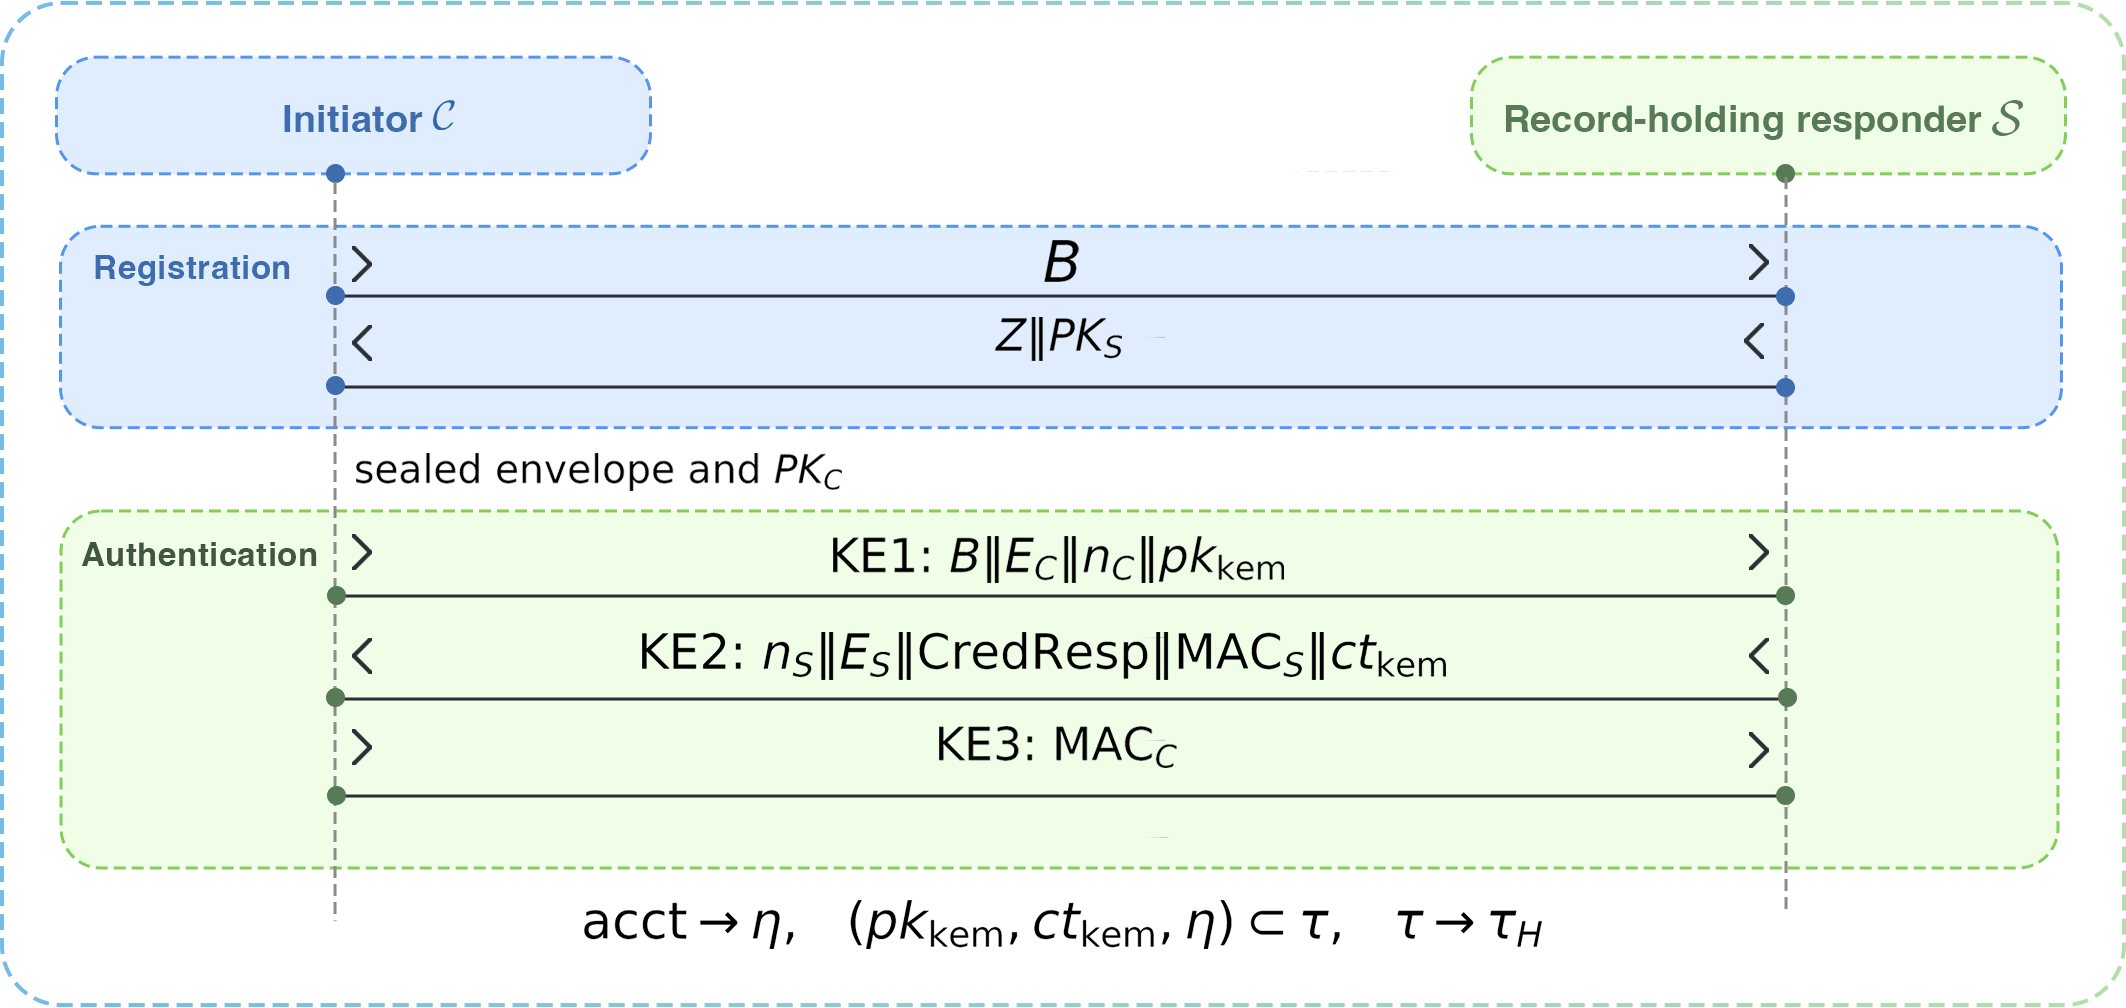
\includegraphics[width=\columnwidth]{figs/figure_2.png}
\caption{Hybrid PQ-OPAQUE authentication flow. The message pattern is unchanged; final key extraction binds the classical 4DH and ML-KEM layers through the transcript.}
\label{fig:acit-flow}
\end{figure}

\subsection{Message Footprint}

The transport consequence of hybridization is concentrated in KE1 and KE2 because those are the messages that carry the ML-KEM public key and ciphertext. KE3 remains essentially unchanged. This asymmetry is operationally favorable: the protocol does not inflate every step uniformly, but only the two messages in which key-establishment material is naturally exchanged.

Concretely, KE1 expands from 88 to 1272 bytes and KE2 from 288 to 1376 bytes, driven respectively by the ML-KEM public key and ciphertext, while KE3 is unchanged at 64 bytes, for a payload total of 2712 bytes. The protocol therefore remains deployable despite a non-trivial increase in message footprint: the message pattern is unchanged, and the additional transport burden appears precisely where the protocol already expects public-key material. With the one-byte version prefix carried by each authentication message, the complete wire-format total becomes 2715~bytes. In many deployment settings, this is materially easier to absorb than an additional round trip or a redesign of the authentication choreography. Figure~\ref{fig:acit-wiregrowth} visualizes where this growth is concentrated.

\begin{figure}[t]
\centering
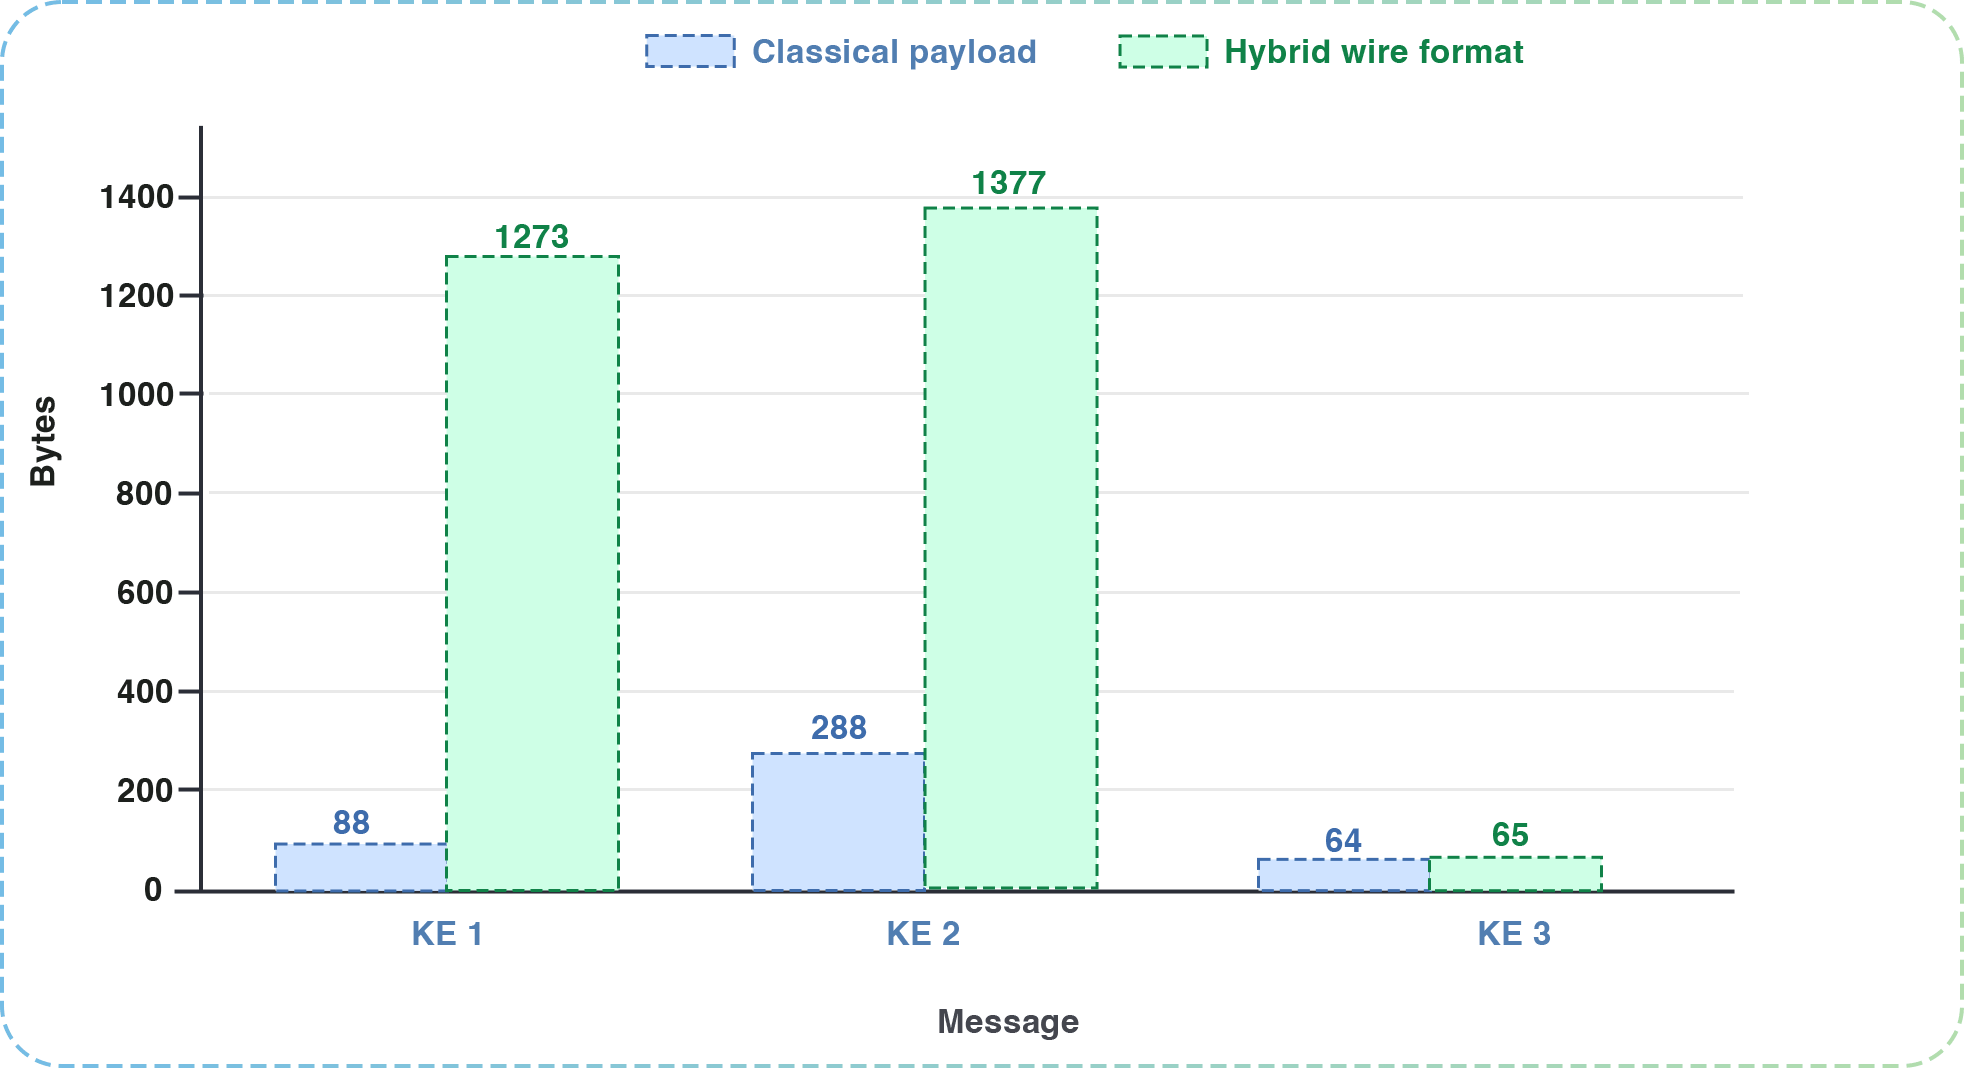
\includegraphics[width=\columnwidth]{figs/figure_3.png}
\caption{Authentication-message size growth from classical to hybrid OPAQUE. The additional payload is concentrated in KE1 and KE2, which carry the ML-KEM public key and ciphertext, while KE3 is unchanged.}
\label{fig:acit-wiregrowth}
\end{figure}

\section{Security Interpretation and Formal Evidence}

The verification and implementation results form a combined evidence base. ProVerif was used in separate secrecy and authentication models; Tamarin was applied to a surrogate 4DH model that abstracts the classical algebraic core; and the implementation was exercised through reproducible tests and benchmarks. The resulting claim is substantial but delimited: it supports the protocol design and observed implementation behavior, not a universal machine proof of every low-level operation \cite{cremers2012,basin2018}.

\subsection{Formal Reading Discipline}

The manuscript does not collapse symbolic verification, executable tests, and performance measurements into one undifferentiated claim. Each layer answers a different methodological question. ProVerif addresses secrecy and correspondence properties in an unbounded-session symbolic setting \cite{blanchet2016}. Tamarin contributes an event-based account of the hybrid combiner, albeit through a surrogate model of the classical 4DH core rather than a low-level account of every group operation \cite{tamarin2013}. The Rust implementation and its regression tests examine whether the design behaves as intended at the level of wire format, protocol state transitions, and error handling.

\begin{table*}[t]
\caption{Symbolic verification summary and modeling boundary {\color{blue}(new)}}
\label{tab:acit-verification}
\centering
\footnotesize
\begin{tabularx}{\textwidth}{@{}L{3.4cm}L{1.9cm}L{2.5cm}X@{}}
\toprule
Property & ProVerif & Tamarin & Modeling boundary \\
\midrule
Session-key secrecy (P1) & confirmed & confirmed (27 steps) & Symbolic secrecy only; no side-channel or compiled-code claim. \\
Password secrecy (P2) & confirmed & confirmed (3 steps) & Checked in the model trace abstraction. \\
Forward secrecy (P3) & not modeled & surrogate (119 steps) & Algebraic forward secrecy rests on Eq.~\eqref{eq:acit-comp-bound}, not on Tamarin. \\
Post-quantum contribution (P4) & not modeled & within surrogate lemma & Not an IND-CCA2 proof of ML-KEM. \\
Initiator authentication (P5a) & confirmed & confirmed (32 steps) & Correspondence under the modeled events. \\
Responder authentication (P5b) & confirmed & confirmed (17 steps) & Correspondence under the modeled events. \\
Injective mutual auth.\ (P5c) & confirmed & on ProVerif side & Not a claim about API misuse or error formatting. \\
Hybrid-source interpretation (P6) & not modeled & surrogate (29 steps) & Evidence for the abstraction, not a combiner theorem. \\
No offline verifier in DB model (P7) & not modeled & supported (4 steps) & Assumes $\sigma_{\mathrm{oprf}}$ stays outside the compromised store. \\
Executability & n/a & confirmed (16 steps) & Confirms an honest completion trace exists. \\
\midrule
Total & 5/5 queries & 8/8 lemmas & Results belong to separate symbolic abstractions. \\
\bottomrule
\end{tabularx}
\end{table*}

Table~\ref{tab:acit-verification} makes the argumentative structure explicit, mapping each property (P1--P7) to its ProVerif and Tamarin status and to the boundary of what the symbolic model does and does not establish. Hybrid security claims are often weakened less by the protocol idea than by ambiguity over which result supports which statement, so the mapping is stated directly: ProVerif discharges five query families---session-key secrecy, password secrecy, initiator and responder authentication, and injective mutual authentication---while Tamarin verifies eight lemmas over the surrogate 4DH model.

No single artifact is treated as dispositive; each addresses a different methodological question, and the final claim is read only through their combined contribution.

\subsection{Detailed Symbolic Coverage}


This addresses a recurring weakness in hybrid papers, where models are presented without a precise statement of what they do and do not support. Here the evidence is partitioned explicitly, and each claim is tied to a specific supporting artifact: session-key secrecy and mutual authentication rest on the ProVerif models, scoped forward secrecy and the combiner interpretation on the Tamarin surrogate, and offline-dictionary resistance only on the OPAQUE-style server-record boundary.

Relative to canonical 3DH-OPAQUE, the construction preserves the three-message, 1.5-round interaction; replaces classical 3DH key-schedule input with 4DH material plus an ML-KEM secret; raises honest-party cost only additively ($+1$~DH, one KEM, $O(1)$); enlarges the handshake by 2272 payload bytes; and, in the adopted model, requires joint weakening of both layers rather than failure of a single classical layer. It also pairs this with multi-source evidence---ProVerif 5/5 queries, Tamarin 8/8 lemmas, and 157 passing tests---whereas prior PAKE papers often omit implementation evidence. The main formal consequence is therefore not a new asymptotic security notion, but a different structure of extractor input under an unchanged operational protocol shape. In canonical 3DH-OPAQUE, the authenticated key exchange depends entirely on classical material. Here, the pseudorandom key in \eqref{eq:hybrid-prk-acit} is bound simultaneously to the classical 4DH layer, the post-quantum KEM secret, and the extended transcript. That change justifies the central comparative statement: under the adopted model, final key recovery requires a materially stronger failure story than in the single-layer classical baseline.

\subsection{\color{blue}Computational Security Argument in the Post-Quantum Model}

\begingroup\color{blue}
Beyond the symbolic models, the hybrid key schedule admits a game-based argument in the post-quantum model that justifies why final-key recovery requires defeating both layers. We state it as a scoped reduction under explicit assumptions rather than as a full universally composable theorem.

The argument relies on three assumptions. First, ML-KEM-768 is IND-CCA2 secure against a quantum-polynomial-time adversary with classical decapsulation-oracle access, so its shared secret $ss_{\mathrm{kem}}$ is indistinguishable from random \cite{fips203}. Second, the classical layer satisfies a Gap-CDH assumption over Ristretto255: recovering the ephemeral term $dh_4$ from the recorded transcript remains hard even given a decisional Diffie--Hellman (DDH) oracle, which the random-oracle reduction needs in order to recognize the adversary's correct Diffie--Hellman value \cite{devalence2024}. Third, HKDF-Extract over HMAC-SHA-512 is modeled, in the (quantum) random-oracle model, as a split-key PRF on the concatenated input under a public, transcript-derived salt, in the sense of the concatenation combiner of Giacon, Heuer and Poettering \cite{giacon2018}.

Let the input keying material be split into a classical part $\mathrm{IKM}_{\mathrm{cl}} = dh_1\|dh_2\|dh_3\|dh_4$ and a post-quantum part $\mathrm{IKM}_{\mathrm{pq}} = ss_{\mathrm{kem}}$, so that the pre-key is $\mathrm{PRK} = \mathrm{HKDF\text{-}Extract}(\mathrm{salt}_\tau,\, \mathrm{IKM}_{\mathrm{cl}}\|\mathrm{IKM}_{\mathrm{pq}})$. Fix a transcript $\tau$. If at least one source---either $\mathrm{IKM}_{\mathrm{pq}}$ or a high-entropy component of $\mathrm{IKM}_{\mathrm{cl}}$ such as $dh_4$---remains computationally hidden and independent of the other conditioned on $\tau$, then by the split-key combiner the extracted key is pseudorandom, and the advantage of any quantum-polynomial-time distinguisher against the session key is bounded by
\begin{equation}
\mathrm{Adv}^{\mathrm{ind}} \le
\min\!\bigl\{
\mathrm{Adv}_{\mathrm{GapCDH}}^{\mathrm{Ristretto255}},\;
\mathrm{Adv}_{\mathrm{ML\text{-}KEM}}^{\mathrm{IND\text{-}CCA2}}
\bigr\}
+ \mathrm{Adv}_{\mathrm{HKDF}}^{\mathrm{skPRF}}.
\label{eq:acit-comp-bound}
\end{equation}

The reduction is the standard concatenation-combiner argument. A distinguisher that separates the real session key from random with advantage $\varepsilon$ is converted, by embedding the IND-CCA2 challenge into $ss_{\mathrm{kem}}$ (or the Gap-CDH challenge into the surviving ephemeral term) and answering HKDF queries through the random oracle, into a distinguisher against the surviving source up to the split-key PRF term \cite{giacon2018,bindel2019}. Against a quantum adversary the same step is read in the quantum random-oracle model, where Grover search only halves the symmetric margins of the 512-bit hash and the 256-bit keys involved, and we rely on the hybrid-KEM QROM analyses for the concatenation pattern \cite{bindel2019}.

The bound \eqref{eq:acit-comp-bound} is deliberately scoped: it models HKDF-Extract in the random-oracle model and does not reprove the OPAQUE-derived password layer, so it complements rather than replaces a universally composable treatment of PAKE \cite{canetti2001}. Within that scope, it is nonetheless a concrete post-quantum security statement: the reinforced session key remains indistinguishable from random as long as \emph{either} the classical Gap-CDH source \emph{or} the post-quantum ML-KEM source survives, which is precisely the guarantee a hybrid migration profile is expected to provide. Figure~\ref{fig:acit-keyschedule} shows the transcript-bound key schedule that underlies this argument.

\begin{figure}[t]
\centering
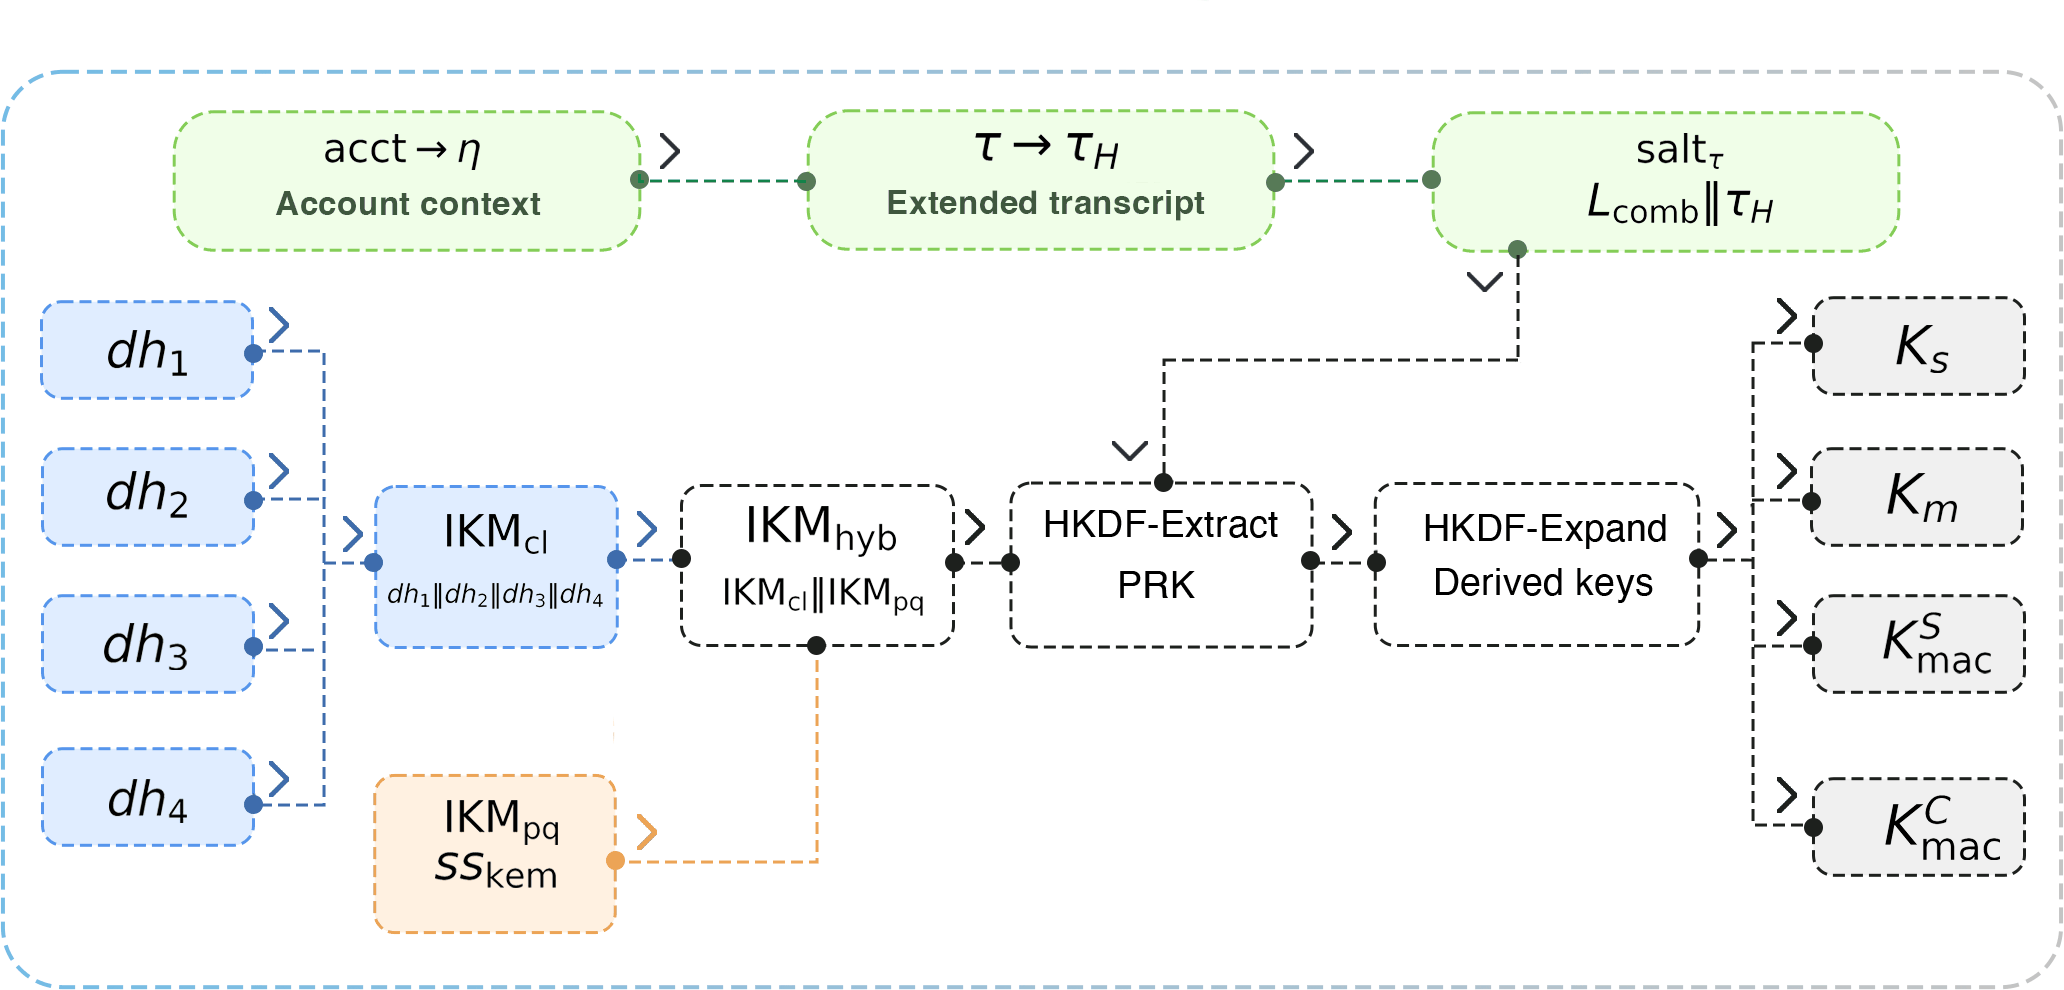
\includegraphics[width=\columnwidth]{figs/figure_4.png}
\caption{\color{blue}Transcript-bound hybrid key schedule. Classical 4DH material and the ML-KEM shared secret are concatenated into a single transcript-salted HKDF-Extract, so the derived keys depend jointly on both layers.}
\label{fig:acit-keyschedule}
\end{figure}
\endgroup

\section{Implementation and Experimental Methodology}

The implementation is reported as a reproducible Rust artifact rather than as pseudocode alone. That choice is methodologically necessary for a hybrid augmented PAKE because many deployment-relevant defects are not mathematical: message framing, state-machine drift between parties, incorrect handling of version markers, unsafe cross-language boundaries, or failure to erase ephemeral material after key derivation. Any deployment-oriented claim that omits these layers leaves too much of the protocol surface unexamined.

The implementation architecture is layered. A cryptographic core provides protocol serialization, transcript processing, and key-derivation logic. Client and server protocol contours build on that core. A narrow foreign function interface (FFI) boundary is used only where low-level interoperability is required. This is not a machine proof of implementation security, but it reduces the number of points at which memory-management defects or inconsistent API semantics can distort the cryptographic design.

\subsection{Artifact Footprint}

The research artifact spans roughly 11{,}000 lines: a 1513-line cryptographic core for key derivation, transcript processing, and serialization; client and server contours of about 900 lines each; a 2026-line FFI layer; 4116 lines of regression, protocol, and interface tests; and 1806 lines of ProVerif and Tamarin models. This breadth is not reported for its own sake; it explains why the argument relies on layered evidence, since a hybrid augmented PAKE simultaneously touches cryptographic routines, protocol choreography, boundary interfaces, and evaluation scripts. Reporting only formal models or only benchmark numbers would conceal that breadth.

\subsection{Memory Safety and Secret Lifecycle}

For a password-authenticated protocol, implementation quality is not determined solely by which primitives are invoked. It also depends on how long sensitive values remain live in memory, whether protocol state can be reused incorrectly, and whether low-level interfaces permit accidental exposure of partially derived secrets. The Rust implementation therefore treats secret lifecycle as a first-class systems property rather than as an afterthought.

Concretely, the initiator path stores DH terms, transcript buffers, PRK material, and the decapsulated ML-KEM secret in zeroizing wrappers, while the responder path explicitly invokes zeroization on classical IKM, MAC inputs, transcript hashes, DH outputs, KEM shared secrets, and retained state on completion, expiry, or authentication failure. At the FFI boundary, handle-owned protocol state is zeroized on drop, and responder-expiry tests assert that private state is cleared after invalidation. These mechanisms do not amount to a full side-channel or compiler-interference proof, but they do define concrete erasure boundaries inside the artifact rather than leaving secret lifecycle as an implicit assumption.


The benchmarking methodology also requires explicit scope. Measurements were taken on a Linux server with two Intel Xeon E5-2650~v4 processors (24 physical cores, 48 hardware threads) and Rust~1.93.1, in optimized runs under Criterion. Criterion reports bootstrap estimates of the mean and the 95\% confidence interval; these values should be read as reproducible platform-specific estimates, not as universal constants. Their value lies in the relative ordering of costs: whether the post-quantum layer is dominant, whether the server-side path remains sub-millisecond, and whether the latency bottleneck remains password hardening. Microbenchmarks and protocol-path benchmarks were collected in separate Criterion scenarios, so the reported means are comparable as profiles rather than as additive components of a single timing equation.

The broader reproducibility point is that no single artifact type is sufficient: a symbolic model can succeed while a wire-format implementation fails, and a clean code base can still overclaim security if its formal scope is unclear, so the artifact layers are designed to reinforce rather than substitute for one another.

\section{Quantitative Results}\label{sec:results}

The measurements support a conservative deployment interpretation. {\color{blue}On the Linux/Xeon platform, the full ML-KEM-768 round costs 336.09~$\mu$s with a 95\% confidence interval of [332.25; 340.43], while isolated server-side KE2 generation remains in the few-hundred-microsecond range. The end-to-end authentication profile is 806.13~ms [797.65; 816.30], but this latency is dominated by Argon2id \cite{argon2rfc2021} rather than by the post-quantum reinforcement itself. Outside password hardening, the reinforcement adds one ML-KEM-768 round (336.09~$\mu$s [332.25; 340.43]) and one extra classical Diffie--Hellman (56.69~$\mu$s), and so remains well below a millisecond.}

\subsection{Selected Microbenchmarks}

\begin{table}[t]
\caption{Selected microbenchmark results {\color{blue}(values on Linux/Xeon platform)}}
\label{tab:acit-microbench}
\centering
\scriptsize
\begin{tabularx}{\columnwidth}{@{}L{1.6cm}L{1.45cm}rY@{}}
\toprule
Primitive & Operation & Mean time & 95\% CI \\
\midrule
Ristretto255 & single DH & 56.69~$\mu$s & [56.29; 57.12] \\
Ristretto255 & 4DH (profile) & 224.23~$\mu$s & [223.09; 225.49] \\
ML-KEM-768 & key generation & 100.72~$\mu$s & [99.96; 101.62] \\
ML-KEM-768 & encapsulation & 103.25~$\mu$s & [98.82; 108.04] \\
ML-KEM-768 & decapsulation & 118.13~$\mu$s & [117.14; 119.23] \\
ML-KEM-768 & full round & 336.09~$\mu$s & [332.25; 340.43] \\
Argon2id & moderate profile & 787.03~ms & [780.86; 793.34] \\
\bottomrule
\end{tabularx}
\end{table}

Table~\ref{tab:acit-microbench} reports the central performance result: the hybrid key-establishment layer remains in the microsecond regime, whereas Argon2id remains in the millisecond regime. The post-quantum cost is therefore additive rather than transformative. The protocol becomes larger on the wire and moderately heavier in the AKE path, but it does not change the dominant latency source.


These headline figures isolate the costs that matter operationally. The end-to-end figure should not be read as post-quantum cryptographic slowdown; the dominant latency source remains password hardening, while the hybrid authenticated key exchange adds only a small amount of extra work in absolute terms. The isolated Argon2id and KE2 measurements characterize where cost resides, not a strict arithmetic decomposition across benchmark harnesses.

\subsection{Protocol-Path Measurements}

\begin{table}[t]
\caption{Protocol-level benchmark scenarios {\color{blue}(values on Linux/Xeon platform)}}
\label{tab:acit-protocol}
\centering
\scriptsize
\begin{tabularx}{\columnwidth}{@{}L{1.35cm}L{1.75cm}rY@{}}
\toprule
Phase & Scenario & Mean time & 95\% CI \\
\midrule
Reg. & request & 114.49~$\mu$s & [113.81; 115.23] \\
Reg. & response & 68.46~$\mu$s & [67.83; 69.17] \\
Reg. & completion & 783.75~ms & [777.98; 790.14] \\
Auth. & KE1 generation & 220.31~$\mu$s & [219.21; 221.80] \\
Auth. & KE2 generation & 557.13~$\mu$s & [547.57; 568.88] \\
Auth. & KE3 at initiator & 784.95~ms & [779.01; 792.64] \\
Full & full cycle & 806.13~ms & [797.65; 816.30] \\
\bottomrule
\end{tabularx}
\end{table}

Table~\ref{tab:acit-protocol} reports the protocol-path measurements, and they show where the engineering budget is spent. Responder-side cryptographic work remains sub-millisecond, which is compatible with server-side scalability. The initiator-side completion path is slower for the same reason as in the classical setting: password hardening dominates the cost profile. KE3 generation and the complete authentication cycle were measured in separate Criterion scenarios with different state-initialization paths, so their means are not additive and need not coincide, although the 95\% confidence intervals overlap. The post-quantum addition changes the composition of authentication only marginally.

This lets us state the main comparative result compactly:
\begin{equation}
\begin{aligned}
C_{\mathrm{hyb}} &= C_{\mathrm{opq}} + C_{\mathrm{1DH}} + C_{\mathrm{KEM}} + O(1), \\
\Delta W_{\mathrm{payload}} &= 2272~\mathrm{bytes}.
\end{aligned}
\label{eq:complexity-acit}
\end{equation}
Equation \eqref{eq:complexity-acit} captures the central systems point: the protocol does not move to a new interaction class, yet it materially hardens the compromise structure in the adopted hybrid model.

Since isolated KE2 generation remains in the few-hundred-microsecond range, the responder path remains compatible with high authentication throughput on commodity hardware. The construction is therefore persuasive not only in end-user latency terms but also in server-provisioning terms, where fixed-round interaction and bounded work per authentication are both valuable.

The security interpretation remains conservative. Claims about offline dictionary resistance are limited to the case in which the attacker compromises the database record but not the root secret from which account-specific OPRF keys are derived. Likewise, the Tamarin result is a surrogate symbolic argument for the hybrid combiner rather than a complete computational proof for every algebraic detail of Ristretto255.

\subsection{Threats to Validity}

The intended reading discipline can be summarized directly. The objective is not to overstate the result, but to state the claim precisely: secrecy and authentication are supported by symbolic models rather than a tight computational reduction; password protection is interpreted for database-record compromise without compromise of the server root secret; the performance profile is reproducible on the Linux/Xeon platform but not claimed as a universal cross-platform bound; and the fixed-round interaction is preserved while transport overhead still has to be absorbed operationally. The work thus contributes an implementation-backed hybridization pattern whose security interpretation is meaningful for systems design while remaining explicit about the abstractions used in symbolic verification and benchmarking.

\section{Deployment Considerations}

The deployment value of a hybrid augmented PAKE depends on more than security semantics. Operators need to know whether the protocol fits existing authentication surfaces, whether server provisioning changes materially, and whether migration can proceed incrementally. The answer here is conservative: the message pattern is preserved, the password-hardening stage remains familiar, and the additional post-quantum cost is concentrated in the authenticated key-exchange portion rather than across the entire account workflow.

The proposal is operationally viable in real systems for a structural reason. The most difficult operational changes in authentication usually arise when a protocol adds a round trip, changes the server-side account model, or imposes substantial cryptographic cost on the hot path. None of those occurs here: no new round trip is introduced, KE2 remains sub-millisecond, client latency stays dominated by Argon2id, and the protocol is introduced as a reinforcement of OPAQUE rather than a replacement of password-authentication logic. The main change is the transport footprint of the first two messages, which is a materially simpler engineering problem than redesigning the authentication choreography.

There is also a sequencing argument for migration. Organizations that already depend on password authentication rarely replace the entire stack in one step. They need transitional designs that can be justified to engineering teams, product owners, and security review boards. A fixed-round hybrid OPAQUE variant fits that setting because the migration path is incremental: preserve the interaction shape, preserve the password-hardening boundary, add a post-quantum layer to the key-establishment core, and validate the result through code and measurements.

\subsection{\color{blue}Scalability in Large Distributed Systems}

\begingroup\color{blue}
Because the construction preserves the fixed-round OPAQUE choreography and introduces no additional round trip, it inherits the horizontal-scaling profile of classical augmented PAKE: stateless front ends and load balancers are unaffected, and authentication can be sharded per account record. The post-quantum material is ephemeral and session-scoped, so it adds no persistent per-account storage and does not enlarge the server-side record that must be replicated across a cluster. On the server hot path, KE2 generation remains sub-millisecond in isolation, so post-quantum key establishment is not the throughput bottleneck even under high authentication load.

The dominant scaling constraint is therefore not the post-quantum layer but the password-hardening stage that the design deliberately leaves unchanged. A 256~MiB Argon2id profile bounds the number of concurrent authentications a node can sustain, because memory rather than CPU saturates first; this constraint is identical to classical OPAQUE and is not introduced by hybridization. In large deployments it is addressed by a dedicated authentication tier, admission control and rate limiting on the login path, and a key-stretching profile tuned to the device class rather than fixed globally. The additional transport cost of $2272$~bytes per authentication, concentrated in KE1 and KE2, scales linearly with the login rate and remains negligible relative to application media traffic, although it should be budgeted explicitly at very high authentication rates. Migrating a large system to Hybrid PQ-OPAQUE therefore changes its memory- and bandwidth-provisioning budget in bounded, predictable ways while leaving its interaction model and scaling topology intact.
\endgroup

The contribution therefore concerns deployment posture as much as protocol composition. The quantitative results show that the cost of hybridization is bounded. The formal results show that the stronger compromise condition is not merely heuristic. The implementation artifact shows that the design withstands serialization, interface boundaries, and regression testing.

\section{Discussion and Conclusion}

Hybrid PQ-OPAQUE shows that post-quantum reinforcement of augmented PAKE can be achieved without increasing round complexity. In the measured implementation, the dominant deployment cost is transport overhead rather than CPU cost: Argon2id remains the latency bottleneck, while the additional authenticated key-exchange work is additive and sub-millisecond. The construction therefore preserves the operational profile of OPAQUE while introducing a bounded and quantified migration cost.

The main scientific point is comparative. Relative to canonical 3DH-OPAQUE, the construction preserves fixed-round interaction, increases honest-party cost only additively, and strengthens the condition for final key recovery in the adopted model. The value of the result lies less in a new asymptotic abstraction than in demonstrating that a strong augmented-PAKE baseline can be hybridized without forfeiting deployment realism.

The claim remains deliberately scoped. It rests on a layered evidence base spanning symbolic analysis, executable code, regression tests, and measurements, and it should be read as an implementation-backed protocol-engineering result rather than as a full computational proof. Under that reading, Hybrid PQ-OPAQUE provides a reproducible and quantitatively characterized fixed-round migration pattern for augmented PAKE.

Natural next steps are equally concrete: a tighter computational treatment of the hybrid combiner and its forward-secrecy boundary, cross-platform measurements under varied Argon2id profiles and transport settings, and broader interoperability checks across independently implemented endpoints. Each would narrow a specific current limitation without altering the central fixed-round engineering result established here.

% \clearpage
% \onecolumn
\section*{ACKNOWLEDGMENT}
OpenAI Codex was used during manuscript preparation to assist with English-language drafting, stylistic revision, and \LaTeX{} editing in portions of the abstract, introduction, discussion, conclusion, and related connective prose. The system was not used as an authoritative source for technical claims. All protocol descriptions, equations, references, tables, implementation details, and experimental results were independently reviewed, verified, and approved by the author.

\begin{thebibliography}{27}

\bibitem{en18071823}
S.~Svystun, L.~Scislo, M.~Pawlik, O.~Melnychenko, P.~Radiuk, O.~Savenko, and A.~Sachenko, ``DyTAM: Accelerating wind turbine inspections with dynamic UAV trajectory adaptation,'' \emph{Energies}, vol.~18, no.~7, p.~1823, 2025. doi:~\url{https://doi.org/10.3390/en18071823}.

\bibitem{Svystun_Melnychenko_Radiuk_Savenko_Sachenko_Lysyi_2024}
S.~Svystun, O.~Melnychenko, P.~Radiuk, O.~Savenko, A.~Sachenko, and A.~Lysyi, ``Thermal and RGB images work better together in wind turbine damage detection,'' \emph{International Journal of Computing}, vol.~23, no.~4, pp.~526--535, Dec. 2024. doi:~\url{https://doi.org/10.47839/ijc.23.4.3752}.

\bibitem{reksreks.2025.2.06}
A.~Lysyi, A.~Sachenko, P.~Radiuk, M.~Lysyi, O.~Melnychenko, O.~Ishchuk, and O.~Savenko, ``Enhanced fire hazard detection in solar power plants: an integrated UAV, AI, and SCADA-based approach,'' \emph{Radioelectronic and Computer Systems}, no.~2, pp.~99--117, 2025. doi:~\url{https://doi.org/10.32620/reks.2025.2.06}.

\bibitem{jarecki2018}
S.~Jarecki, H.~Krawczyk, and J.~Xu, ``OPAQUE: An asymmetric PAKE protocol secure against pre-computation attacks,'' in \emph{EUROCRYPT 2018}, LNCS~10822, pp.~456--486, 2018. doi:~\url{https://doi.org/10.1007/978-3-319-78372-7_15}.

\bibitem{ietf-opaque}
D.~Bourdrez, H.~Krawczyk, K.~Lewi, and C.~A.~Wood, ``The OPAQUE Augmented Password-Authenticated Key Exchange (aPAKE) Protocol,'' RFC~9807, Jul.~2025. Available:~\url{https://www.rfc-editor.org/info/rfc9807}.

\bibitem{ladd2023}
W.~Ladd, ``SPAKE2, a password-authenticated key exchange,'' RFC~9382, Sep.~2023. Available:~\url{https://www.rfc-editor.org/info/rfc9382}.

\bibitem{spake2plus2023}
T.~Taubert and C.~A.~Wood, ``SPAKE2+, an Augmented Password-Authenticated Key Exchange (PAKE) Protocol,'' RFC~9383, Sep.~2023. Available:~\url{https://www.rfc-editor.org/info/rfc9383}.

\bibitem{mosca2018}
M.~Mosca, ``Cybersecurity in an Era with Quantum Computers: Will We Be Ready?,'' \emph{IEEE Security \& Privacy}, vol.~16, no.~5, pp.~38--41, Sep./Oct.~2018. doi:~\url{https://doi.org/10.1109/MSP.2018.3761723}.

\bibitem{shor1994}
P.~W.~Shor, ``Algorithms for quantum computation: discrete logarithms and factoring,'' in \emph{Proceedings of the 35th Annual Symposium on Foundations of Computer Science}, 1994, pp.~124--134. Expanded version available:~\url{https://arxiv.org/abs/quant-ph/9508027}.

\bibitem{bernstein2017}
D.~J.~Bernstein and T.~Lange, ``Post-quantum cryptography,'' \emph{Nature}, vol.~549, no.~7671, pp.~188--194, 2017. doi:~\url{https://doi.org/10.1038/nature23461}.

\bibitem{roetteler2017}
M.~Roetteler, M.~Naehrig, K.~M.~Svore, and K.~Lauter, ``Quantum resource estimates for computing elliptic curve discrete logarithms,'' in \emph{ASIACRYPT 2017}, LNCS~10625, pp.~241--270, 2017. doi:~\url{https://doi.org/10.1007/978-3-319-70697-9_9}.

\bibitem{babbush2026}
R.~Babbush, A.~Zalcman, C.~Gidney, M.~Broughton, T.~Khattar,
H.~Neven, T.~Bergamaschi, J.~Drake, and D.~Boneh,
``Securing elliptic curve cryptocurrencies against quantum vulnerabilities:
Resource estimates and mitigations,'' arXiv:2603.28846, Mar.~2026.
doi:~\url{https://doi.org/10.48550/arXiv.2603.28846}.

\bibitem{fips203}
National Institute of Standards and Technology, ``Module-Lattice-Based Key-Encapsulation Mechanism Standard,'' FIPS~203, Aug.~2024. doi:~\url{https://doi.org/10.6028/NIST.FIPS.203}.

\bibitem{fips204}
National Institute of Standards and Technology, ``Module-Lattice-Based Digital Signature Standard,'' FIPS~204, Aug.~2024. doi:~\url{https://doi.org/10.6028/NIST.FIPS.204}.

\bibitem{canetti2001}
R.~Canetti, ``Universally composable security: A new paradigm for cryptographic protocols,'' in \emph{Proceedings of the 42nd IEEE Symposium on Foundations of Computer Science}, 2001, pp.~136--145. Full version available:~\url{https://eprint.iacr.org/2000/067}.

\bibitem{tlshybrid2025}
D.~Stebila, S.~Fluhrer, and S.~Gueron, ``Hybrid key exchange in TLS 1.3,'' Internet-Draft draft-ietf-tls-hybrid-design-16, Sep.~2025. Work in progress. Available:~\url{https://datatracker.ietf.org/doc/draft-ietf-tls-hybrid-design/}.

\bibitem{devalence2024}
H.~de~Valence, J.~Grigg, M.~Hamburg, I.~Lovecruft, G.~Tankersley, and F.~Valsorda, ``The ristretto255 and decaf448 groups,'' RFC~9496, Dec.~2023. Available:~\url{https://www.rfc-editor.org/info/rfc9496}.

\bibitem{krawczyk2010}
H.~Krawczyk and P.~Eronen, ``HMAC-based extract-and-expand key derivation function (HKDF),'' RFC~5869, May~2010. Available:~\url{https://www.rfc-editor.org/info/rfc5869}.

\bibitem{cremers2012}
C.~Cremers and S.~Mauw, \emph{Operational Semantics and Verification of Security Protocols}. Springer, 2012. doi:~\url{https://doi.org/10.1007/978-3-540-78636-8}.

\bibitem{basin2018}
D.~Basin, C.~Cremers, and C.~Meadows, ``Model checking security protocols,'' in \emph{Handbook of Model Checking}, Springer, 2018, pp.~727--762. doi:~\url{https://doi.org/10.1007/978-3-319-10575-8_22}.

\bibitem{blanchet2016}
B.~Blanchet, ``Modeling and verifying security protocols with the applied pi calculus and ProVerif,'' \emph{Foundations and Trends in Privacy and Security}, vol.~1, nos.~1--2, pp.~1--135, 2016. Available:~\url{https://bblanche.gitlabpages.inria.fr/publications/BlanchetFnTPS16.pdf}.

\bibitem{tamarin2013}
S.~Meier, B.~Schmidt, C.~Cremers, and D.~Basin, ``The TAMARIN prover for the symbolic analysis of security protocols,'' in \emph{CAV 2013}, LNCS~8044, pp.~696--701, 2013. doi:~\url{https://doi.org/10.1007/978-3-642-39799-8_48}.

\bibitem{argon2rfc2021}
A.~Biryukov, D.~Dinu, D.~Khovratovich, and S.~Josefsson, ``Argon2 memory-hard function for password hashing and proof-of-work applications,'' RFC~9106, Sep.~2021. Available:~\url{https://www.rfc-editor.org/info/rfc9106}.

\bibitem{bellovin1992}
S.~M.~Bellovin and M.~Merritt, ``Encrypted key exchange: password-based protocols secure against dictionary attacks,'' in \emph{Proc.\ IEEE Symp.\ Security and Privacy}, 1992, pp.~72--84. doi:~\url{https://doi.org/10.1109/RISP.1992.213269}.

\bibitem{wu1998}
T.~Wu, ``The secure remote password protocol,'' in \emph{Proc.\ Network and Distributed System Security Symp.\ (NDSS)}, 1998, pp.~97--111.

\bibitem{giacon2018}
F.~Giacon, F.~Heuer, and B.~Poettering, ``KEM combiners,'' in \emph{Public-Key Cryptography -- PKC 2018}, LNCS~10769, pp.~190--218, 2018. doi:~\url{https://doi.org/10.1007/978-3-319-76578-5_7}.

\bibitem{bindel2019}
N.~Bindel, J.~Brendel, M.~Fischlin, B.~Goncalves, and D.~Stebila, ``Hybrid key encapsulation mechanisms and authenticated key exchange,'' in \emph{Post-Quantum Cryptography -- PQCrypto 2019}, LNCS~11505, pp.~206--226, 2019. doi:~\url{https://doi.org/10.1007/978-3-030-25510-7_12}.

\end{thebibliography}

\end{document}
